\section{Introduction}
\label{sec:intro}

%{\em
%``The goal is to turn data into information, and information into insight.''}
%\vspace{-5pt}
%\begin{flushright}
%--- Carly Fiorina
%\end{flushright}

%Recent interest on geometry processing has been moving towards high-level understanding and intelligent processing of
%three dimensional shapes, with a general goal of discovering patterns about their compositions and structures,
%and relating structures with semantic meanings and functionalities.
%This momentum gives rise to the recent topic of structure-aware geometry processing~\cite{Mitra:2014:SASP}.
%Shape structure implies human knowledge about 3D shapes in terms of part configurations.
%Thus, a natural approach to structural shape analysis and structure-aware shape processing is knowledge-driven,
%where structure is extracted, interpreted and represented with domain-specific knowledge incorporated.
%Examples are like minima-rule-based heuristics for shape segmentation~\cite{Shamir:2008:SMS}, procedural models~\cite{Muller:2006:PMB}
%and rule-based generative models~\cite{Merrell:2011:IFL} for 3D shape modeling.
Recent interest on geometry processing of three dimensional shapes and scenes has been moving into developing algorithms that learn from data to intelligently
perform high-level tasks of understanding and processing, and automatically produce results that are comparable to those that would be produced by humans with tedious manual effort.
The general theme of these methods is to discover patterns about the geometry and structure of shapes and scenes, and relate them
to high-level concepts, semantics, function and models that explain these patterns. In contrast to traditional approaches in geometry processing, these methods do not treat shapes and scenes
in complete isolation of each other, and do not rely on manually tuned and explicitly programmed instructions.
Instead, they jointly analyze several shapes to extract and model meaningful mappings and correlations in the data to make useful predictions.

In retrospect, the idea of utilizing existing shapes to support geometry processing has been exploited and practiced for many years.
However, most early works based on such idea are confined with the example-based paradigm, where the core concept is \emph{information transfer}.
Typically, the input to these problems include one or multiple source/exemplar shapes possessing prescribed or pre-computed information of interest,
as well as a target shape being analyzed or processed. The task is to build a \emph{correlation} between the source and target shapes so that
the interesting information can be transferred from source to target. The applications of such approach range from
%texture synthesis~\cite{Wei:2009:EBT},
shape analysis (e.g.~\cite{Schaefer:2007:EBS}) to shape synthesis (e.g.~\cite{Ma:2014:ADS}), etc.

When the number of involved 3D shapes becomes significantly large, however, geometry processing supported by existing data has been fundamentally changed.
Besides information transfer, several new concepts emerge with new applications.
As the amount of 3D models continues to grow, the rich variability of 3D content in existing shape repositories makes it possible to directly reuse the shapes
or parts for constructing new shapes~\cite{Funkhouser:2004:MBE}. Such \emph{content reuse} for 3D modeling is perhaps the most straightforward consequence of big 3D geometric data,
providing a promising approach to addressing the well-known 3D content creation bottleneck.
More importantly, high-level understanding of shapes can be achieved via co-analyzing collections of shapes, which is based on
a premise that shape understanding can only be reliable by observing a set of semantically related shapes instead of a single observation.
To achieve \emph{co-analysis}, a critical step is to find the correlation between the multiple shapes in the input set, where the problem is substantially different from that in building pair-wise correlation. A key concept here is \emph{consistency} of the correlations among the entire set, with both mathematic description~\cite{Huang:2013:SDP} and semantic interpretation~\cite{Wang:2012:ACS}.


\paragraph*{From knowledge-driven to data-driven.}
A common approach to high-level shape understanding is knowledge-driven,
where geometric and structural patterns are extracted and interpreted with rules or parameters specified explicitly by humans.
Examples are like heuristics based shape analysis and procedural shape modeling.
%and rule-based generative models (e.g.,~\cite{Merrell:2011:IFL}).
Although being successful in many problems, the inherent limitations of knowledge-driven approach have restrained its application in more complex tasks.
The first and foremost difficulty is that it is often uneasy to turn human knowledge
into useful rules and relevant parameters used to model process of 3D shape understanding.
%This is especially challenging for the task of shape understanding.
%Human cognition about shapes and structures is mainly based on visual perception involving the grouping of individual elements into coherent patterns~\cite{Murray:2002:SPR}.
%It is difficult to compile such visual perception activities into formulism of guidelines or constraints.
Secondly, human experience and judgement are usually formed with limited observations which often
can not generalize well for large data. Such generalization issue is more notable for
3D shapes, especially those of man-made objects, which exhibit significant variations on both geometry and topology
even within the same shape category.%~\cite{Xu:2010:SCS,Wang:2012:ACS}.

Data driven modeling, on the other hand, learns the models and/or parameters from large amount of observed data.
Its main advantage is the less dependence on prior knowledge, and consequently less reliance on hand-crafted models/parameters, making it more data-adaptive and generalizable.
The success of data-driven approach, underlaid by machine learning techniques, relies heavily on the accessibility of large data collections.
It is showed that increasing the training set by orders of magnitude yields significant performance improvements for common machine learning algorithms~\cite{Banko:2001:MPA}.
With the recent developments in 3D modeling tools and acquisition techniques for 3D geometry,
many large repositories of 3D shapes (e.g. Trimble 3D Warehouse, Aim at Shape etc.) have emerged.
The availability of such large data collections has aroused significant interest on
data-driven approach to 3D shape analysis and processing, and greatly stimulated its development in recent years.


\paragraph*{Relation with structure-aware shape processing.}
This report is closely related to the recent excellent survey on ``structure-aware shape processing'' by Mitra and co-workers~\cite{Mitra:2014:SASP},
which concerns about works on structural analysis of 3D shapes, as well as high-level shape processing constrained with structure-preservation.
In their work, shape structure is defined as the arrangement and relations between shape parts,
which is analyzed through identifying shape parts, part parameters, and part relations.
Each of the three can be determined through manual assignment, predefined model fitting and data-driven learning.

Our report focuses on the line of research on data-driven geometry processing which stands well on itself as an independent direction.
\emph{Firstly}, data-driven shape processing frequently goes beyond structure analysis.
For example, large shape collections may benefit more diverse problems in shape understanding and processing,
such as parametric modeling of shape space~\cite{Allen:2003:SHB,Kalogerakis:2009:DDC},
hypothesis generation for object and scene understanding~\cite{Zia:2013:DR,Satkin:2012:DDS},
and information transfer between multi-modal data~\cite{Wang:2013:PAS,Su:2014:EID}.
Meanwhile, data-driven shape processing may also exploit the data-centered techniques in machine learning
such as sparse coding~\cite{Ren:2013:HSC} and feature learning~\cite{Lai:2013:UFL},
which are not pre-conditioned on any domain-specific or structural prior beyond raw data.
%
\emph{Secondly}, even within the realm of structure-aware shape processing, data-driven approach is becoming a dominant branch due
to its theoretical and practical advantages, and the availability of large shape repositories and the fast development of machine learning techniques.

\section{Overview}
\label{sec:overview}

In this section, we provide a high-level overview of the main components and steps of data-driven approaches for processing 3D shapes and scenes. Although the pipeline of these methods vary significantly depending on their particular applications and goals, a number of components tend to be common: the input data collection and processing, data representations and feature extraction, as well as learning and inference. \emph{Representation, learning and inference} are critical components of machine learning approaches in general \cite{Koller:2009:PGM}. In the case of shape and scene processing, each of these components poses several interesting and unique problems when dealing with 3D geometric data. These problems have greatly motivated the research on data-driven geometry processing, and in turn have brought new challenges to the computer vision and machine learning communities, as reflected by the increased interest in 3D visual data from these fields. Below, we discuss particular characteristics and challenges of data-driven 3D shape and scene processing algorithms.
\rev{Figure~\ref{fig:overview} provides a schematic overview of the most common components of these algorithms.}

\begin{figure*}[t!]
\centering
    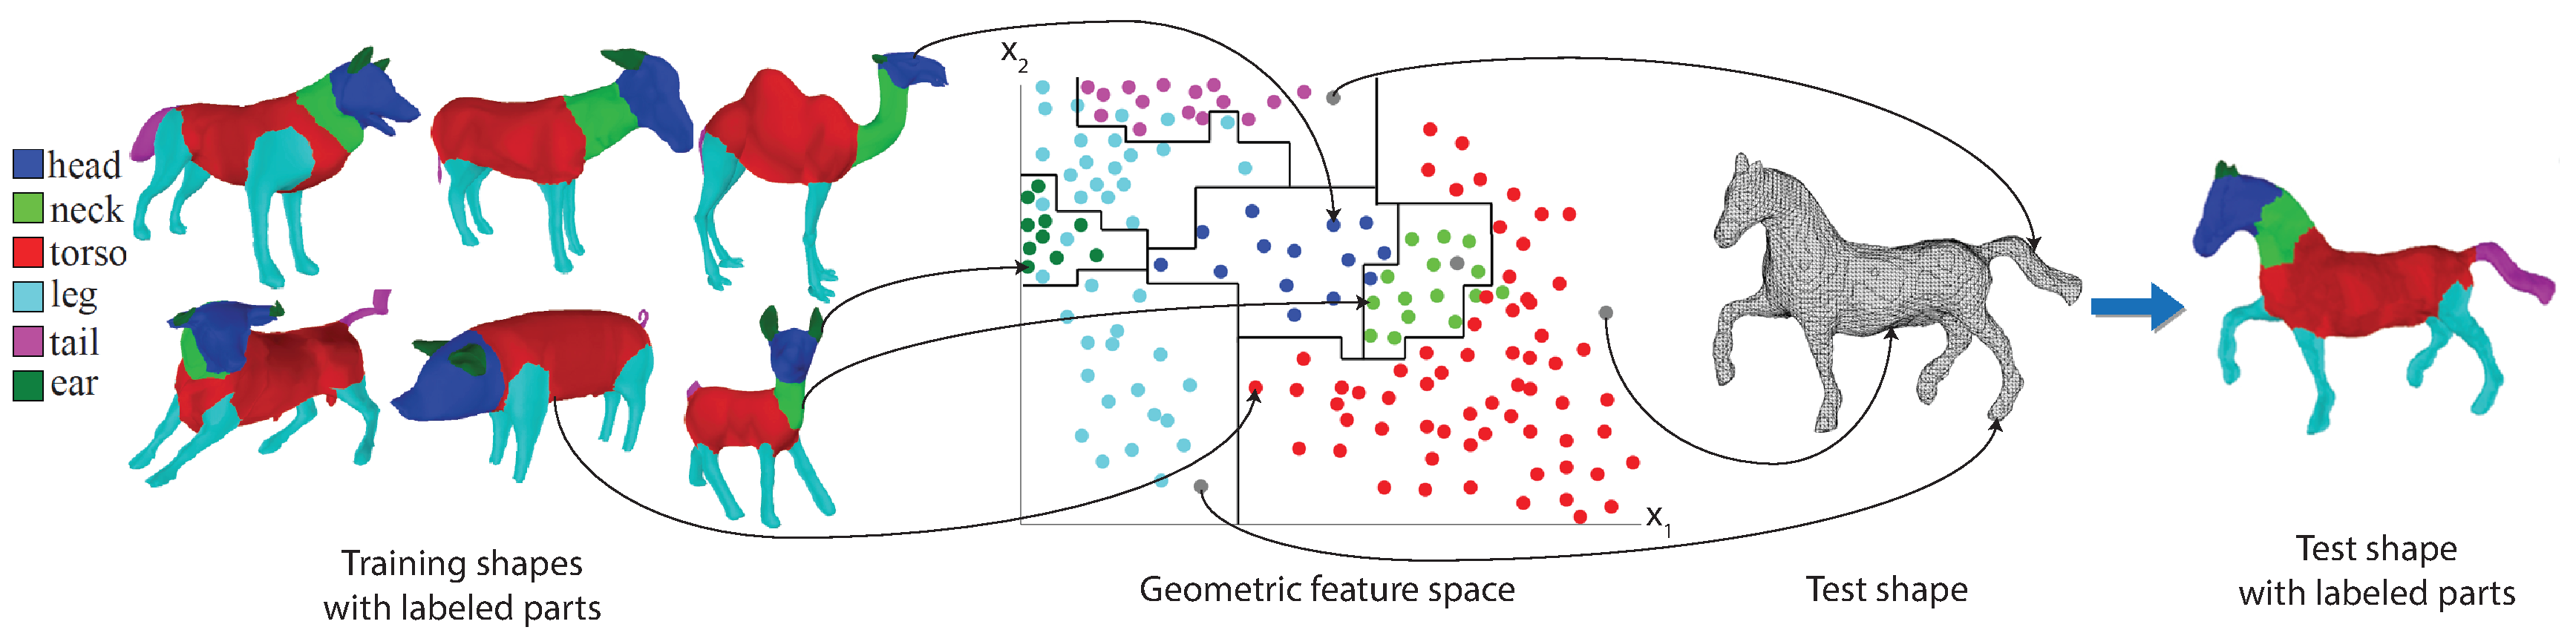
\includegraphics[width=1.0\textwidth]{fig/img/overview_seg.pdf}
    %\vspace{-.5cm}
    \caption{
Pipeline of a supervised segmentation algorithm \cite{Kalogerakis:2010:LMS}. Given a set of shapes with labeled parts, the points of each shape are embedded in a common feature space based on their local geometric descriptors (a color is assigned to points depending on their given part label). A classifier is learned to split the feature space into regions corresponding to each part label. Given a test shape, its points (shown in grey) are first embedded in the same space. Then part labels are inferred for all its points based on the learned classifier and an underlying structured probabilistic model (Section \ref{sec:segmentation}).
}
\label{fig:overview_seg}
\end{figure*}



\subsection{3D data collection}

\para{Shape representation.} A main component of data-driven approaches for shape and scene processing is data collection, where the goal is acquire a number of 3D shapes and scenes depending on the application. When shapes and scenes are captured with scanners or depth sensors, their initial representation is in the form of \emph{range data} or \emph{unorganized point clouds}. Several data-driven methods for reconstruction, segmentation and recognition directly work on these representations and do not require any further processing. On the other hand, online repositories, such as the Trimble 3D Warehouse, contain millions of shapes and scenes that are represented as \emph{polygon meshes}. A large number of data-driven techniques are designed to handle complete shapes in the form of polygon meshes created by 3D modeling tools or re-constructed from point clouds. Choosing which representation to use depends on the application. For example, data-driven reconstruction techniques aim for generating complete shapes and scenes from noisy point clouds with missing data. The reconstructed shapes can then be processed with other data-driven methods for categorization, segmentation, matching and so on. Developing methods that can handle any 3D data representation, as well as jointly reconstructing and analyzing shapes is a potential direction for future research we discuss in Section \ref{sec:conclusion}.

When polygon meshes are used as the input representation, an important aspect to consider is whether and how data-driven methods will deal with possible ``defects'', such as non-manifold and non-orientable sets of polygons, inverted faces, isolated elements, self-intersections, holes and topological noise. The vast majority of meshes available in online repositories have these problems. Although there is a number of mesh repairing tools (see \cite{Campen:PGP:2012} for a survey), they may not handle all different types of ``defects'', and can take a significant amount of time to process each shape in a large dataset. To avoid the issues caused by these ``defects'', some data-driven methods uniformly sample the input meshes and work on the resulting point-based representation instead (e.g., \cite{Chaudhuri:2011:prabm,Kim:2013:lpt}).

\paragraph*{Datasets.} Although it is desirable to develop data-driven methods that can learn from a handful of training shapes or scenes, this is generally a challenging problem in machine learning \cite{Fei:OSL:2006}. Several data-driven methods in computer vision have been particularly successful due to the use of very large datasets that can reach the size of several millions of images \cite{Torralba:2008:MTI}. In contrast, data-driven approaches for 3D shape and scene processing approaches have mostly relied on datasets that reach the order of a few thousands so far (e.g., Princeton Shape Benchmark \cite{Shilane:2004:TPS}, or datasets collected from the web \cite{Kim:2013:lpt}). Online repositories contain large amount of shapes, which can lead to the development of methods that will leverage datasets that are orders of magnitudes larger than the ones currently used.
%
\fix{One significant example is the recently available ShapeNet~\cite{Shapenet}, which provides a richly-annotated, large-scale dataset of 3D shapes.
Similar to ImageNet, a well-known image database in the computer vision community, ShapeNet is organized based on the WordNet hierarchy.
It has indexed about 3 million models, out of which 220 thousand models are classified into 3,135 WordNet synsets (a synset refers to a meaningful concept in WordNet).}

Another possibility is to develop synthetic datasets. A notable example is the pose and part recognition algorithm used in Microsoft's Kinect that relies on 500K synthesized shapes of human bodies in different poses \cite{Shotton:2011:RLH}. In general, large datasets are important to capture the enormous 3D shape and scene variability, and can significantly increase the predictive performance and usability of learning methods. A more comprehensive summary of existing online data collections can be found on our wikipage~\cite{Wikipage}.


\subsection{3D data processing and feature representation}
It is common to perform some additional processing on the input representations of shapes and scenes before executing the main learning step. The reason is that the input representations of 3D shapes and scenes can have different resolutions (e.g., number of points or faces), scale, orientation, and structure. In other words, the input shapes and scenes do not initially have any type of common parameterization or alignment. This is significantly different from other domains, such as natural language processing or vision, where text or image datasets frequently come with a common parameterization beforehand (e.g., images with the same number of pixels and objects of consistent orientation).

To achieve a common parameterization of the input shapes and scenes, one popular approach is to embed them in a \emph{common geometric feature space}. For this purpose a variety of shape descriptors have been developed. These descriptors can be classified into two main categories: \emph{global shape descriptors} that convert each shape to a feature vector,  and \emph{local shape descriptors} that convert each point to a feature vector. Examples of global shape descriptors are Extended Gaussian Images \cite{Horn:1984:EGI}, 3D shape histograms \cite{Ankerst:1999:3dsh,Chaudhuri:2010:DDS}, spherical functions \cite{Saupe:2001:MRS}, lightfield descriptors \cite{Chen:2003:ovsb}, shape distributions \cite{Osada:2002:sd}, symmetry descriptors \cite{Kazhdan:2004:SD3D}, spherical harmonics \cite{Kazhdan:2003:RISH}, 3D Zernicke moments \cite{Novotni:2003:3DZD}, and bags-of-words created out of local descriptors \cite{Bronstein:2011:SGGW}. Local shape descriptors include surface curvature, PCA descriptors, local shape diameter \cite{Shapira:2008:SDF}, shape contexts \cite{Belongie:2002:SMO,Kalogerakis:2010:LMS,Kokkinos:2012:ISC}, spin images \cite{Johnson:1999:USI}, geodesic distance features \cite{Zhang:2005:FSP}, heat-kernel descriptors \cite{Bronstein:2011:SGGW}, and depth features \cite{Shotton:2011:RLH}. Global shape descriptors are particularly useful for shape classification, retrieval and organization. Local shape descriptors are useful for partial shape matching, segmentation, and point correspondence estimation. Before using any type of global or local descriptor, it is important to consider whether the descriptor will be invariant to different shape orientations, scales, or poses. In the presence of noise and irregular mesh tessellations, it is important to robustly estimate local descriptors, since surface derivatives are particularly susceptible to surface and sampling noise \cite{Kalogerakis:2007:RSE}. It is also possible to use several different descriptors as input, and let the learning step decide which ones are more relevant for each class of shapes \cite{Kalogerakis:2010:LMS}.

\fix{
A different approach, which has attracted large attention in the computer vision community, is to avoid manually engineered features and instead directly learn features them from raw data. This approach has been enlightened by the recent developments in deep learning~\cite{Bengio:2009:LDA,Yu:FLI:2010}, and in particular Convolutional Neural Networks (CNNs) \cite{Krizhevsky:ICDL:2012,Szegedy:GDC:2015}.
A number of deep learning architectures have been recently proposed to learn 3D shape and scene descriptors, operating on either voxel-based representations \cite{Wu:3SN:2015}, view-based projections \cite{Su:MCN:2015,Xie:PFL:2015}, spectral representations \cite{Boscaini:2015:LCS}, or RGB-D data ~\cite{Socher:2012:CRD,Blum:2012:LFD,Lai:2013:UFL,Bo:2014:LHS}.}

Instead of embedding shapes in a common geometric feature space, several methods instead try to directly align shapes in Euclidean space. We refer the reader to the survey on dynamic geometry processing for a tutorial on rigid and non-rigid registration techniques \cite{Chang:DGP:2012}. An interesting extension of these techniques is to include the alignment process in the learning step of data-driven methods, since it is inter-dependent with other shape analysis tasks such as shape segmentation and correspondences \cite{Kim:2013:lpt}.

Some data-driven methods require additional processing steps on the input. For example, learning deformation handles or fully generative models of shapes usually rely on segmenting the input shapes into parts with automatic algorithms \cite{Huang:2011:JSS,Sidi:2011:CS} and representing these parts with surface abstractions \cite{Yumer:2012:CSC} or descriptors \cite{Kalogerakis:2012:PMC}. To decrease the amount of computation required during learning, it is also common to represent the shapes as a set of patches (super-faces) \cite{Huang:2011:JSS} inspired by the computation of super-pixels in image segmentation.

\subsection{Learning and Inference}
The processed representations of shapes and scenes are used to perform learning and inference for a variety of applications: shape classification, segmentation, matching, reconstruction, modeling, synthesis, and scene analysis. The learning procedures significantly vary depending on the application, thus we discuss them individually in each of the following sections on these applications. As a common theme, learning is viewed as an \emph{optimization} problem that runs on a set of variables representing geometric, structural, semantic or functional properties of shapes and scenes. There is usually a single or multiple objective (or loss) functions for quantifying preferences for different models or patterns governing the 3D data. After learning a model from the training data, inference procedures are used to predict values of variables for new shapes or scenes. Again, the inference procedures vary depending on the application, and are discussed separately in the following sections. It is common that inference itself is an optimization problem, and sometimes is part of the learning process when there are latent variables or partially observed input shapes or scene data.

A general classification of the different types of algorithms used in data-driven approaches for shape and scene processing can be derived from the type of input information available during learning:

\begin{itemize}
\item \textbf{Supervised learning} algorithms are trained on a set of shapes or scenes annotated with labeled data. For example, in the case of shape classification, these labeled data can have the form of tags, while in the case of segmentation, the labeled data have the form of segmentation boundaries or part labels. The labeled data can be provided by humans or generated synthetically. After learning, the learned models are applied on different sets of shapes (test shapes) to produce results relevant to the task.
\item \textbf{Unsupervised} algorithms co-analyze the input shapes or scenes without any additional labeled data i.e., the desired output is unknown beforehand. The goal of these methods is to discover correlations in the geometry and structure of the input shape or scene data. For example, unsupervised shape segmentation methods usually perform some type of clustering in the feature space of points or patches belonging to the input shapes.
\item \textbf{Semi-supervised} algorithms make use of shapes (or scenes) with and without any labeled data. Active learning is a special case of semi-supervised learning in which a learning algorithm interactively queries the user to obtain desired outputs for more data points related to shapes.
\end{itemize}

In general, supervised methods tend to output results that are closer to what a human would expect given the provided labeled data. However, they may fail to produce desirable results when the training shapes (or scenes) are geometrically and structurally dissimilar from the test shapes (or scenes). They also tend to require a substantial amount of labeled information as input, which can become a significant burden for the user. Unsupervised methods can deal with collections of shapes and scenes with larger variability and require no human supervision. However, they sometimes require parameter tuning to yield the desired results. Semi-supervised methods represent a trade-off between supervised and unsupervised methods: they provide more direct control to the user about the desired result compared to unsupervised methods, and often produce considerable improvements in the results by making use of both labeled and unlabeled shapes or scenes compared to supervised methods.


\paragraph*{The data-driven loop.}
An advantageous feature of data-driven shape processing is that the output data, produced by learning and inference, typically come with rich semantic information.
For example, data-driven shape segmentation produces parts with semantic labels~\cite{Kalogerakis:2010:LMS}; data-driven reconstruction is commonly coupled with semantic part or shape recognition~\cite{Shen:2012:SRP,Nan:2012:SAC}; data-driven shape modeling can generate readily usable shapes inheriting the semantic information from the input data~\cite{Xu:2011:PMO}.
These processed and generated data can be used to enrich the existing shape collections with both training labels and reusable contents, which in turn benefit subsequent learning. In a sense,
data-driven methods \emph{close the loop of data generation and data analysis} for 3D shapes and scenes; see Figure~\ref{fig:overview}.
\rev{Such concept has been practiced in several prior works, such as the data-driven shape reconstruction framework proposed in~\cite{Pauly:2005:ESC} (Figure~\ref{fig:pauly_sgp05_esr}).}

\paragraph*{Pipeline example.}
To help the reader grasp the pipeline of data-driven methods, a schematic overview of the components is given in Figure \ref{fig:overview}.
Depending on the particular application, the pipeline can have several variations, or some components might be skipped. We discuss the main components and steps of algorithms for each application in more detail in the following sections. A didactic example of the pipeline in the case of supervised shape segmentation is shown in Figure \ref{fig:overview_seg}. The input shapes are annotated with labeled part information. A geometric descriptor is extracted for each point on the training shapes, and the points are embedded in a common feature space. The learning step uses a classification algorithm that non-linearly separates the input space into a set of regions corresponding to part labels in order to optimize classification performance (more details are provided in Section \ref{sec:segmentation}). Given a test shape, a probabilistic model is used to infer part labels for each point on that shape based on its geometric descriptor in the feature space.

\subsection{A comparative overview}
\rev{Before reviewing the related works in detail, we provide a comparative overview of them
in Table~\ref{tab:compare}, and correlate them under a set of \emph{criteria}:
\begin{itemize}
  \item \textbf{Training data.} Data-driven methods can be categorized according to the
 shape or scene  representations they operate on, the scale (size) of
the training datasets they use, and the type of pre-processing applied to these datasets.
                                The most common representation for shapes are polygon
meshes and point clouds. 3D scenes are typically represented as an arrangement of
                                individual shapes, usually organized in a scene graph.
                                Pre-processing includes pre-segmentation, over-segmentation, pre-alignment, initial correspondence, or/and labeling.
  \item \textbf{Features.} Roughly speaking, there are two types of feature representations involved in data-driven shape processing.
                          The most commonly used feature representations are low-level ones, such as local geometric features (e.g., local curvature)
                          and global shape descriptors (e.g. shape distribution~\cite{Osada:2002:sd}). If the input shapes are pre-segmented into meaningful parts, high-level structural
                          representations (spatial relationships of parts) can be derived. Generally, working with high-level feature representations enables the learning of more powerful models
                          for more advanced inference tasks, such as structural analysis~\cite{Mitra:2014:SASP}, on complex man-made objects and scenes.
  \item \textbf{Learning model/approach.} The specific choice of learning method is often application-dependent. In most cases,  machine learning techniques are adapted
or developed from scratch to
                                          process geometric data. For some problems, such as shape correspondence, the core problem is to extract geometric correlations
                                          between different shapes in an unsupervised manner, which itself can be seen as a learning problem specific to geometry processing.
  \item \textbf{Learning type.} As discussed above, there are three basic types of data-driven methods, depending on the use of labeled training data:
                                supervised, semi-supervised and unsupervised methods.
  \item \textbf{Learning outcome.} Learning can produce different types of outputs:
parametric or non-parametric models (classifiers, clusterings, regressors, etc.),
                                   distance metrics which can be utilized for further analysis, and/or feature representations learned from raw data.
  \item \textbf{Application.} The main applications of data-driven shape analysis and processing include classification, segmentation, correspondence,
                              modeling, synthesis, reconstruction, exploration and organization.
\end{itemize}}

%Data is to the center of machine learning, which often determines the specific learner to be utilized.
%Regardless of the learning mechanism, the success of data-driven shape processing depends directly on the quality of the training data.
%A quality dataset should be large and dense to sufficiently cover the shape variability within the corresponding categories.
%Individually, each shape should possess adequate quality in terms of geometric completeness and tropologic cleanness, to enable correct shape characterization.
%For supervised learning, the shapes in the collection should also be correctly segmented and labeled.
%The scant availability of large collections ofquality and/or labeled 3D shapes constitutes the \emph{data challenge} for data-driven shape processing.

%3D shapes are typically represented as surface or volumetric representation.
%These structure-oblivious representations are suitable for the estimation of local or low-level geometric properties, but not for
%attributing shapes with semantics or functionalities.
%A structure-aware representation should be part-based~\cite{Mitra:2014:SASP}.
%Many works has been devoted to the co-analysis of a set of semantically related shapes, leading to consistent segmentation of the set.



%Most existing learning algorithms are devised for 2D vision data; transiting these frameworks to adapt to 3D geometric data is absolutely non-trivial.
%A common solution is to embed 3D shapes or shape parts into some feature space defined for 3D geometry, so that standard data analysis
%such as clustering, dimension reduction, feature selection can be performed in the feature space.
%On the other hand, some works directly perform shape space analysis.




%\item \textbf{Data collection.}
%Data is to the center of machine learning, which often determines the specific learner to be utilized.
%Regardless of the learning mechanism, the success of data-driven shape processing depends directly on the quality of the training data.
%A quality dataset should be large and dense to sufficiently cover the shape variability within the corresponding categories.
%Individually, each shape should possess adequate quality in terms of geometric completeness and tropologic cleanness, to enable correct shape characterization.
%For supervised learning, the shapes in the collection should also be correctly segmented and labeled.
%The scant availability of large collections ofquality and/or labeled 3D shapes constitutes the \emph{data challenge} for data-driven shape processing.
%%
%\item \textbf{Data representation.}
%3D shapes are typically represented as surface or volumetric representation.
%These structure-oblivious representations are suitable for the estimation of local or low-level geometric properties, but not for
%attributing shapes with semantics or functionalities.
%A structure-aware representation should be part-based~\cite{Mitra:2014:SASP}.
%Many works has been devoted to the co-analysis of a set of semantically related shapes, leading to consistent segmentation of the set.
%%
%\item \textbf{Feature space analysis.}
%Most existing learning algorithms are devised for 2D vision data; transiting these frameworks to adapt to 3D geometric data is absolutely non-trivial.
%A common solution is to embed 3D shapes or shape parts into some feature space defined for 3D geometry, so that standard data analysis
%such as clustering, dimension reduction, feature selection can be performed in the feature space.
%On the other hand, some works directly perform shape space analysis.
%%
%\item \textbf{Data assumptions vs. learning models.}
%Different assumptions over the input datasets, e.g. pre-segmentation, pre-alignment, correspondence, and labels
%determine the specific choice of learning models, as well as the methods for training and inference.
%For example,
%%a learning model can work at face level, superface level, or part level of 3D surface shapes.
%%Working at a finer level usually leads to more find-grained analysis but less efficient algorithms.
%depending on the availability of labels, unsupervised, supervised and semi-supervised learning methods can be utilized.
%In general, the more assumptions are employed, the less flexible the model is.
%To the extreme, some models assume no prior knowledge other than data related assumptions, such as smoothness, manifold and cluster.
%\end{itemize}
%
%\paragraph*{Types of models}
%Parametric models:
%
%Generative models including bla bla
%
%Inverse procedural models.
%
%\paragraph*{Problems benefiting from data-driven}
%List all the problems.
%
%
%\subsection{Example: Data-driven mesh segmentation and labeling}
%\label{subsec:example1}
%Talk about the skeleton of the basic approach. And discuss a minimal example.
%\kai{Vangelis?}
%
%\subsection{Example: Data-driven shape reconstruction}
%\label{subsec:example1}
%\kai{Peter?}





%In this section, we provide a high-level overview of data-driven approach to geometry processing and geometric modeling.
%To set the stage, we will begin with a brief review of the general data-driven approach widely applied in many disciplines.
%Then we discuss its application in geometry processing, while setting up the scope of our report.
%Specifically, we will first introduce the specific data processed in geometry processing.
%The major data-driven models utilized in such circumstance are discussed.
%Based on that, we provide categorization method for the existing large amount of related works.
%At last, we will also provide two mini-examples extracted from typical applications of data-driven approach in geometry processing,
%to provide the reader with an intuitive understanding of the general approach.
%
%\subsection{Data-driven modeling approach}
%Data-driven approach is a general paradigm of modeling real world systems based on observed data.
%The overall goal of data-driven modeling is to extract information or knowledge from a data set
%and model the knowledge with to support high level applications of data processing and understanding.
%In a broad sense, the main pipeline of data-driven approaches follows that of machine learning,
%including data preprocessing, model learning and inference.
%
%\subsection{Data-driven models in geometry processing}
%\label{subsec:data}
%Data-driven approach encompasses several major components,
%such as data collection, data representation, feature extraction, as well as model designing, training and inference.
%Each of these components poses many interesting and unique problems when dealing with 3D geometric data.
%These problems have greatly motivated the research on data-driven geometry processing,
%and in turn bought new challenges to the computer vision and machine learning communities, as reflected by the increasing interest in 3D visual data from these fields.
%\begin{itemize}


%\item \textbf{Data collection.}
%Data is to the center of machine learning, which often determines the specific learner to be utilized.
%Regardless of the learning mechanism, the success of data-driven shape processing depends directly on the quality of the training data.
%A quality dataset should be large and dense to sufficiently cover the shape variability within the corresponding categories.
%Individually, each shape should possess adequate quality in terms of geometric completeness and tropologic cleanness, to enable correct shape characterization.
%For supervised learning, the shapes in the collection should also be correctly segmented and labeled.
%The scant availability of large collections ofquality and/or labeled 3D shapes constitutes the \emph{data challenge} for data-driven shape processing.
%%
%\item \textbf{Data representation.}
%3D shapes are typically represented as surface or volumetric representation.
%These structure-oblivious representations are suitable for the estimation of local or low-level geometric properties, but not for
%attributing shapes with semantics or functionalities.
%A structure-aware representation should be part-based~\cite{Mitra:2014:SASP}.
%Many works has been devoted to the co-analysis of a set of semantically related shapes, leading to consistent segmentation of the set.
%%
%\item \textbf{Feature space analysis.}
%Most existing learning algorithms are devised for 2D vision data; transiting these frameworks to adapt to 3D geometric data is absolutely non-trivial.
%A common solution is to embed 3D shapes or shape parts into some feature space defined for 3D geometry, so that standard data analysis
%such as clustering, dimension reduction, feature selection can be performed in the feature space.
%On the other hand, some works directly perform shape space analysis.
%%
%\item \textbf{Data assumptions vs. learning models.}
%Different assumptions over the input datasets, e.g. pre-segmentation, pre-alignment, correspondence, and labels
%determine the specific choice of learning models, as well as the methods for training and inference.
%For example,
%%a learning model can work at face level, superface level, or part level of 3D surface shapes.
%%Working at a finer level usually leads to more find-grained analysis but less efficient algorithms.
%depending on the availability of labels, unsupervised, supervised and semi-supervised learning methods can be utilized.
%In general, the more assumptions are employed, the less flexible the model is.
%To the extreme, some models assume no prior knowledge other than data related assumptions, such as smoothness, manifold and cluster.
%\end{itemize}
%
%\paragraph*{Types of models}
%Parametric models:
%
%Generative models including bla bla
%
%Inverse procedural models.
%
%\paragraph*{Problems benefiting from data-driven}
%List all the problems.
%
%
%\subsection{Example: Data-driven mesh segmentation and labeling}
%\label{subsec:example1}
%Talk about the skeleton of the basic approach. And discuss a minimal example.
%\kai{Vangelis?}
%
%\subsection{Example: Data-driven shape reconstruction}
%\label{subsec:example1}
%\kai{Peter?}


\paragraph*{Vision and motivation.}
In many fields of computer science, data-driven approach is a timely topic under the background of ``big data''.
Although 3D geometry data is still far from being ubiquitous as compared to other data like photographs, the fast growing amount of 3D models and the recent trend of fusing 2D and 3D data have made the era of ``big visual data'' more expectable than ever. Especially in recent, the invention of commodity RGB-D camera has opened the door to low-cost, universal acquisition of 3D data, and brought new possibilities for connecting 2D and 3D data. The connection of 2D and 3D data will provide much more enriched data sources for data-driven methods.

On the other hand, data-driven approach, augmented with existing 3D data collections, will in turn benefit the recognition and reconstruction of acquired 3D data, as well as the synthesis of new shapes. These newly generated data typically come with rich semantic information produced by data-driven inference, which will enhance exiting shape collections with both reusable content and training labels.
In summary, data-driven geometry processing will close the loop from acquisition, analysis, processing to generation of 3D shapes (see Figure~\ref{fig:overview}), and will play a major role in the realization of big visual data.

Recent years have witnessed a fast development of the research on data-driven geometry processing, from both computer graphics and computer vision communities, as reflected by the large body of ever-growing related works. Given the wide attention and interest, the new concepts and unique problems, as well as the new applications and potential opportunities, we believe this direction deserves a comprehensive and systematic survey.

\paragraph*{Organization.}
This survey is organized as follows. Section~\ref{sec:overview} gives a high-level overview of the general data-driven approach and discusses the specific problems of data-driven methods when dealing with 3D geometric data. The section also provides two typical mini-examples for the reader to understand the general work-flow of data-driven geometry processing. The following sections survey the various data-driven shape processing problems in detail, with the critical problems and concepts explained and discussed. Finally, we conclude by listing a set of key challenges and providing a vision on future opportunities.

\paragraph*{Accompanying online resources.}
In order to assist the readers to learn the basic algorithms through exploring existing resources, we provide an online wikipage~\cite{Wikipage}, collecting tools, source codes, together with test data for typical problems and applications on data-driven shape processing. This page will also maintain, or link to, many large data collections for both shapes and scenes, with proper classification and informative instructions. The website could serve as a starting point for those who are conducting research in this direction and possibly, and benefit a wider spectrum of researchers from related fields. 